%!TEX root = paper.tex
\chapter{The pipeline}
\label{sec:overview}

\begin{figure}
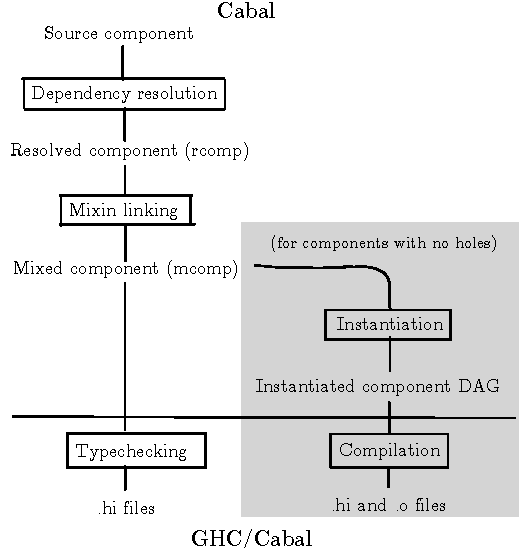
\includegraphics{diagrams/pipeline.pdf}
\caption{Diagram of the pipeline}\label{fig:pipeline}
\end{figure}

\begin{figure}
\begin{mdframed}
\begin{description}
    \item[Source component]
        The smallest unit of user-written source which can have its
        dependencies resolved, e.g., a library, an executable or a test
        suite.  A \textbf{source package} contains one or more source
        components, and is the unit of code that may be distributed
        (e.g., on Hackage).  A source package is identified by a
        \textbf{package identifier} consisting of a package name and
        package version (e.g., \verb|p-0.1|); a source component is in
        turn identified by a \textbf{source component identitifer}
        consisting of the package identifier with the name of the
        component.
    \item[\Ccomp{}] ($\Scomp$ in Figure~\ref{fig:rcomponents}) The output of dependency
        resolution on a source component.  A \ccomp{} is the
        input source with direct dependencies resolved to
        other \ccomp{}s, and \Backpack{}-irrelevant Cabal fields dropped.
        As dependency resolution is
        nondeterministic, a \ccomp{} is identified by a \textbf{\cid}
        ($p$), which augments the source component identifier with the
        resolved \cid{}s of the direct dependencies.  (Thus, the \cid{}
        identifies the entire transitive source a component depends on.)
        In \Backpack{}, we can treat \cid{}s as opaque strings.
    \item[\Unit{}] ($\Uunit$ in Figure~\ref{fig:lcomponents}) The output
        of mixin linking on a \ccomp{}, where we have computed the ``wiring
        diagram'' for the direct dependencies of the unit, describing how
        requirements of the \ccomp{}'s direct dependencies have been
        (partially) filled.  Mixin linking is
        deterministic; thus, a \unit{} is also identified by a \cid{}.  A
        \unit{} can be typechecked by the compiler.
%   \item[Instantiated component]  The output of instantiating a
%       \unit{}.  It is identified by an \textbf{\uid{}} ($P, Q ::= \I{p}[S]$,
%       also known as a \emph{unit identifier})
%       which is simply a \cid{} equipped with a module substitution.
%       If the substitution has no module holes, an instantiated component
%       can be compiled; otherwise, the type of an instantiated component
%       can be computed by appropriately substituting over the type of the \unit{}.  Two types are equivalent if and only if
%       they are defined by the same module from the same \unit{}s instantiated in the same
%       way.
%   \item[Module substitution] ($S ::= \overline{m \mapsto M}$)  A module substitution
%       is a mapping from module names to module identifiers.  These are most
%       commonly used to say how a component is instantiated.
%   \item[Module name] ($m$) Source-level module name, e.g., \verb|Data.Map|.
%   \item[Module identifier] ($M ::= P\!:\!m \,|\, \holevar{m}$)  A fully
%       qualified name (by $P$) for a module, or a module hole
%       $\holevar{m}$ (which can be instantiated by filling the
%       requirement at $m$).
\end{description}
\caption{Glossary of representations in \Backpack{}}
\label{fig:glossary}
\end{mdframed}
\end{figure}

\newsavebox{\resolvedfullexample}
\begin{lrbox}{\resolvedfullexample}
\hspace{-1em}
\begin{minipage}{\linewidth}
\begin{alltt}
component db-dsl-1.0-aaa
 backpack-include: base-4.7-bbb (Prelude)
 required-signature: Data.ByteString
 required-signature: Db
 exposed-module: DSL.Db

component mysql-indef-1.0-ccc
 backpack-include: base-4.7-bbb (Prelude)
 required-signature: Data.ByteString
 exposed-module: Db.MySQL

component mysql-dsl-indef-1.0-ddd
 backpack-include: base-4.7-bbb (Prelude)
 backpack-include: db-dsl-1.0-aaa (DSL.Db) requires (Db)
 backpack-include: mysql-indef-1.0-ccc (Db.MySQL as Db)
 required-signature: Data.ByteString
 reexported-module: DSL.Db as DSL.Db.MySQL
\end{alltt}
\end{minipage}
\end{lrbox}

\begin{figure}
    \usebox{\resolvedfullexample}
  \caption{\Ccomp{}s for \texttt{mysql-dsl-indef-1.0}.}%
\label{fig:resolved-full-comps}
\end{figure}

%   The problem we are trying to solve 

%   The primary contribution of \Backpack{} is to separate mixin linking and
%   typechecking against interfaces: mixin linking 

%   Enough syntax, time to explain how it all works.  In Figure~\ref{fig:pipeline}, 

The implementation and semantics of \Backpack{} is structured as a
series of passes (Figure~\ref{fig:pipeline}) on several intermediate
languages (Figure~\ref{fig:glossary}).  The key idea is that some of
these passes can be performed solely by the package manager, without
inspecting any Haskell code.  In this section, we will give a detailed
summary of all the phases in this pipeline, starting with the source
package language described in the previous section, and continuing on to
two intermediate languages that will serve as the basis for our
semantic account for \Backpack{}.  Our running example will be a
simplified version of the final example from the tour (Figure~\ref{fig:composing-requirements}), shown in Figure~\ref{fig:stuff}.

% \begin{figure}
% \[
% \begin{array}{rcl}
% m & & \mbox{Module name} \\
% p, q & & \mbox{\Cid} \\[0.3em]
% \Uhsbody & & \mbox{Module source} \\
% \Uhssig & & \mbox{Signature source} \\
% \Scomp & ::= & \Scomponent{\Up}{\overline{\Sdecl}} \\[0.3em]
% \Sdecl & ::= & \Sinclude{\Up}{\I{rns}} \\
%        & |   & \Sexposed{m}{\Uhsbody} \\
%        & |   & \Sother{m}{\Uhsbody} \\
%        & |   & \Sreexported{m}{m'} \\
%        & |   & \Srequired{m}{\Uhssig} \\
% \I{rns} & ::= & [\Slparen\overline{rn}\Srparen]~[\texttt{requires}~ \Slparen\overline{rn'}\Srparen] \\
% \I{rn} & ::= & \Sas{m}{m'} \\
%        & |   & m \\
% \end{array}
% \]
% \caption{Syntax of \ccomp{}s}
% \label{fig:rcomponents}
% \end{figure}

% \begin{figure}
% \begin{verbatim}
% component db-dsl-1.0
%   include: base-4.7 (Prelude)
%   required-signature: Data.ByteString
%   required-signature: Db
%   exposed-module: DSL.Db

% component mysql-indef-1.0
%   include: base-4.7 (Prelude)
%   required-signature: Data.ByteString
%   exposed-module: Db.MySQL

% component mysql-dsl-indef-1.0
%   include: base-4.7 (Prelude)
%   include: db-dsl-1.0 (DSL.Db) requires (Db)
%   include: mysql-indef-1.0 (Db.MySQL as Db)
%   required-signature: Data.ByteString
%   reexported-module: DSL.Db as DSL.Db.MySQL
% \end{verbatim}
% \caption{\Ccomp{}s for \texttt{mysql-dsl-indef-1.0}.  In this example,
% we've elided source code for signatures and modules and simplified the
% \cid{}s: in reality, they must record the versions of the dependencies
% they transitively depend on (usually a hash.) \Scott{It might help to
% add ``library'' to sample component names to emphasize that these result
% from resolving the ``library'' component of the packages. Or maybe this
% should just be mentioned somewhere.}}
% \label{fig:resolved-full-example}
% \end{figure}

% \begin{figure}
% \hspace{-0.5em}\begin{verbbox}
% component base
%   exposed-module: W
%                          component r
% component p                include: base (W)
%   required-signature: A    include: p (Y) requires (B)
%   required-signature: B    include: q (X as B)
%   exposed-module: Y        required-signature: A
%                            reexported-module: Y as Z
% component q
%   required-signature: A
%   exposed-module: X
% \end{verbbox}
% \theverbbox{}\\
% \caption{Running example, a more compact version of Figure~\ref{fig:resolved-full-example}.
% The source code is still elided.  By convention, $A, B, C$ are signatures and $X, Y$ are modules.}
% \label{fig:resolved-example}
% \end{figure}

% \begin{figure}
% \[
% \begin{array}{rcrcl}
% \cidl{base} &\haspr& \lctxpairex{\provMod{W}{\icid{base}{}}{W}}{} \\
% \cidl{p} &\haspr& \lctxpairex%
%     {%
%         \provMod{Y}{%
%             \icid{\cidl{p}}{ \subst{A}{\holevar{A}}, \subst{B}{\holevar{B}}  }%
%         }{Y}%
%     }%
%     {\modname{A}, \modname{B}} \\
% \cidl{q} &\haspr& \lctxpairex{\provMod{X}{\icid{\cidl{q}}{\subst{A}{\holevar{A}}}}{X}}%
%                              {\modname{A}} \\
% \cidl{r} &\haspr&
%     \lctxpairex{\provMod{Z}{\icid{\cidl{p}}{%
%                         \subst{A}{\holevar{A}},
%                         \substMod{B}{\icid{\cidl{q}}{\subst{A}{\holevar{A}}}}{X}
%                     }}{Y}}%
%                {\modname{A}} \\
% \end{array}
% \]
% \caption{Component shape for running example.}
% \label{fig:running-shape}
% \end{figure}


\subsection{Dependency resolution to a \ccomp{}}

The first step in
processing a source component is \emph{dependency resolution},
the existing Cabal phase that
selects the versions and conditional flags of all direct dependencies of
a source component (and their transitive direct dependencies as well).
For example, Figure~\ref{fig:resolved-full-comps} shows the results
of resolving a few examples from the tour, with each component renamed to
a \cid{}, which records the name, version, and a hash (e.g., \verb|aaa|)
recording how its direct dependencies were resolved to \cid{}s.

The result of dependency resolution is a \emph{\ccomp}
(Figure~\ref{fig:rcomponents}) which has all conditionals and fields
irrelevant to \Backpack{} eliminated, and all direct dependencies
resolved to \cid{}s.  A \ccomp{} is precisely the fragment of the
Cabal package language which is relevant to \Backpack{}, written in a
form convenient for processing (e.g., each \verb|exposed-module| is
specified individually and explicitly associated with its source).

Dependency resolution in Cabal is a separate topic in its own
right~\cite{well-typed-solver, well-typed-qualified}, beyond the scope of this paper.
Instead, we simply assume that we have a black box which
produces \ccomp{}s.  However, we do have to mention one thing about resolution:
how are \verb|build-depends| fields from
a source component translated into \verb|backpack-include| fields in the
\ccomp{}?  For any package \verb|p|
mentioned in \verb|build-depends| that is not mentioned in
\verb|backpack-includes|, it simply translates to
\verb|backpack-include: p|.
% If a package from \verb|build-depends| is not mentioned
% by \verb|backpack-includes|, it gets given a default \verb|include: p|
% declaration; otherwise, the \verb|backpack-includes| field translates
% directly to a series of \verb|include| statements.

%!TEX root = paper.tex

\newcommand{\figsep}{\vspace*{.2cm}\textcolor{gray}{\rule{\linewidth}{.25pt}}}
\newcommand{\capsep}{\vspace*{.2cm}}%\rule{\linewidth}{.5pt}}

\begin{figure}
    \[
    \begin{array}{rcl}
    m & & \mbox{Module name} \\
    p, q & & \mbox{\Cid} \\[0.3em]
    \Uhsbody & & \mbox{Module source} \\
    \Uhssig & & \mbox{Signature source} \\
    \Scomp & ::= & \Scomponent{\Up}{\overline{\Sdecl}} \\[0.3em]
    \Sdecl & ::= & \Sinclude{\Up}{\I{rns}} \\
           & |   & \Sexposed{m}{\Uhsbody} \\
           & |   & \Sother{m}{\Uhsbody} \\
           & |   & \Sreexported{m}{m'} \\
           & |   & \Srequired{m}{\Uhssig} \\
    \I{rns} & ::= & [\Slparen\overline{rn}\Srparen]~[\texttt{requires}~ \Slparen\overline{rn'}\Srparen] \\
    \I{rn} & ::= & \Sas{m}{m'} \\
           & |   & m \\
    \end{array}
    \]
    \caption{\Ccomp{}s.}
    \label{fig:rcomponents}
\end{figure}

\begin{figure}

    \[
    \begin{array}{lcll}
    \lctx & ::= & \lctxpairx{\provs}{\reqs} & \mbox{Component shape} \\
    %r_\textsf{R} & ::= & \overline{m \rightarrow m'} & \mbox{Requirement renaming (total)} \\
    %r_\textsf{P} & ::= & \overline{m \rightarrow m'} & \mbox{Provision renaming (partial)} \\
    \reqs  & ::= & \overline{\hv{m}} & \mbox{Required module variables} \\
    \provs & ::= & \overline{\prov{m}{M}}  & \mbox{Provided modules} \\
    \shctx & ::= & \overline{\Up \shapeis \lctx} & \mbox{Component shape context} \\
    \end{array}
    \]
    \[
    \begin{array}{rcll}
      M   &::=& \Mod{\UP}{m} & \text{Module identity} \\
          &|&   \holevar{m} & \text{Module hole} \\
      \UP &::=& \icid{\Up}{S} & \text{\Uid} \\
      S   &::=& \overline{\subst{m}{M}} & \text{Module substitution} \\
    \end{array}
    \]
    \[
    \begin{array}{rcll}
      \Uunit &::=& \UsynUnit{\Up}{\reqs}{\overline{\Uudecl}} & \text{Mixed component} \\
      \Uudecl &::=& \UsynDep{\UP}{r} & \text{Direct dependency} \\
              &|&   \UsynMod{m}{\Uhsbody} & \text{Module definition} \\
              &|&   \UsynSig{m}{\Uhssig} & \text{Signature definition} \\
              %& &   \qquad \textsf{with}~\overline{P\!:\!m} & \quad\text{(Merges)} \\
              %&|&   \UsynLet{m}{M} & \text{Let binding} \\
      %\mprog &::=& \overline{\Uunit} & \text{Mixed program} \\
      r   &::=& \overline{m \mapsto m'} & \text{Module renaming} \\
    \end{array}
    \]

\caption{Component shapes and \unit{}s.}
\label{fig:lcomponents}
\end{figure}



\begin{figure}
\begin{verbatim}

component p                 component base
 required-signature: A       exposed-module: W
 required-signature: B
 exposed-module: Y          component q
                             required-signature: A
component r                  exposed-module: X
 required-signature: A
 mixin: base (W)
 mixin: p (Y) requires (B)
 mixin: q (X as B)
 reexported-module: Y as Z
\end{verbatim}
  \caption{Heavily simplified version of Figure~\ref{fig:resolved-full-comps} to serve as the running example: \texttt{p} is \texttt{db-dsl}, \texttt{q} is \texttt{mysql-indef} and \texttt{r} is \texttt{mysql-dsl-indef}; signature \texttt{A} is \texttt{Data.ByteString} and signature \texttt{B} is \texttt{Db}.}
  \label{fig:resolved-example}
\end{figure}

\begin{figure}
    \[
    \begin{array}{l}
      \UsynUnitH{\cidl{base}}{} \haspr \{\provMod{W}{\icid{base}{}}{W}\}  \\
      %\quad \UsynLet{W}{\Mod{\icid{base}{}}{W}} \\
      \quad \UsynMod{\modname{W}(\texttt{I}(..))}{\texttt{data I = MkI I; f (MkI i) = i}} \\
      \\
      \UsynUnitH{\cidl{p}}{\hv{\modname{A}}~\hv{\modname{B}}}
        \haspr \{
            \provMod{Y}{%
                \icid{\cidl{p}}{ \subst{A}{\holevar{A}}, \subst{B}{\holevar{B}}  }%
            }{Y} \} \\
      \quad \UsynSig{A}{\texttt{data J}} \\
      \quad \UsynSig{B}{\texttt{data K}} \\
      %\quad \UsynLet{Y}{\MOD{p}{\substHole{A}, \substHole{B}}{Y}} \\
      \quad \UsynMod{Y}{\texttt{import A; import B; data L = MkL J K}} \\
      \\
      \UsynUnitH{\cidl{q}}{\hv{\modname{A}}}
        \haspr \{ \provMod{X}{\icid{\cidl{q}}{\subst{A}{\holevar{A}}}}{X} \}
      \\
      \quad \UsynSig{\modname{A}~(\texttt{I}(..))}{\texttt{data I = MkI I}} \\
      %\quad \UsynLet{X}{\MOD{q}{\substHole{A}}{X}} \\
      \quad \UsynMod{\modname{X}~(\texttt{I}(..), \texttt{K}(..))}{\texttt{import A; data K = MkK I}} \\
      \\
      \UsynUnitH{\cidl{r}}{\hv{\modname{A}}}
        \haspr \{
        \provMod{Z}{\icid{\cidl{p}}{%
                 \subst{A}{\holevar{A}},
                 \substMod{B}{\icid{\cidl{q}}{\subst{A}{\holevar{A}}}}{X}
             }}{Y} \}
        \\
      \quad \UsynDep{\icid{base}{}}{ \rename{W}{W} } \\
      \quad \mathsf{signature}~\modname{A}~(\texttt{I}(..))~\{ \texttt{import W(I(..))} \} \\
      %\quad\quad \textsf{with}~\Mod{\icid{\cidl{q}}{\substHole{A}}}{A},
      %           \Mod{\icid{\cidl{p}}{\substHole{A}, \subst{B}{\ldots}}}{A} \\
      \quad \UsynDep{\icid{\cidl{q}}{\substHole{A}}}{ \rename{X}{B} } \\
      \quad \UsynDep{\icid{\cidl{p}}{\substHole{A}, \substMod{B}{\icid{\cidl{q}}{\substHole{A}}}{X}}}{ \rename{Y}{Y} } \\
    \end{array}
    \]

  \caption{\Unit{}s. Each component is ordered and annotated with its provided modules, as
    $\textsf{component}~p~\overline{\protect\hv{m}}\haspr\{\provs\}$.}
  \label{fig:linked-example}
\end{figure}

\begin{figure}
    \[
    \begin{array}{l}
    \cidl{base}
        : \left\{\right\} \rightarrow
          \left\{
            \modname{W}
            : \begin{array}{l}
                \UobjIface\: (\MOD{base}{}{W}.\texttt{I}, \MOD{base}{}{W}.\texttt{f} ) \\
                \quad\texttt{data I :: * = MkI}\ \MOD{base}{}{W}.\texttt{I} \\
                \quad\texttt{f ::}~\MOD{base}{}{W}.\texttt{I}~\rightarrow~\MOD{base}{}{W}.\texttt{I}
            \end{array}
          \right\}
    \\[2em]
    \cidl{p} : \forall \hv{A} \hv{B}.\, \forall \nhv{\texttt{A.J}} \nhv{\texttt{B.K}}. \\
    \quad
    \left\{
        \modname{A}
          : \begin{array}{l}
                \UobjIface\: (\nhv{\texttt{A.J}}) \\
                \quad\texttt{data J :: *}
            \end{array},\,
        \modname{B}
          : \begin{array}{l}
                \UobjIface\: (\nhv{\texttt{B.K}}) \\
                \quad\texttt{data K :: *}
            \end{array}
    \right\}
    \rightarrow \\
    \quad
    \left\{
        \modname{Y}
          : \begin{array}{l}
                \UobjIface\: (\MOD{p}{\substHole{A}, \substHole{B}}{Y}.\texttt{L}) \\
                \quad\texttt{data L :: * = MkL \nhv{\texttt{A.J}} \nhv{\texttt{B.K}}}
            \end{array}
    \right\}
    \\[2em]
    \cidl{q} : \forall \hv{A}.\, \forall \nhv{\texttt{A.I}}. \\
    \quad
    \left\{
        \modname{A}
          : \begin{array}{l}
                \UobjIface\: (\nhv{\texttt{A.I}}) \\
                \quad\texttt{data I :: * = MkI}\ \nhv{\texttt{A.I}}
            \end{array}
    \right\}
    \rightarrow \\
    \quad
    \left\{
        \modname{X}
          : \begin{array}{l}
                \UobjIface\: (\nhv{\texttt{A.I}}, \MOD{q}{\substHole{A}}{X}.\texttt{K}) \\
                \quad\texttt{data K :: * = MkK \nhv{\texttt{A.I}}}
            \end{array}
    \right\}
    \\[2em]
    \cidl{r} : \forall \hv{A}.\, \forall \nhv{\texttt{A.J}}. \\
    \quad
    \left\{
        \modname{A}
          : \begin{array}{l}
                \UobjIface\: (\MOD{base}{}{W}.\texttt{I}, \nhv{\texttt{A.J}}) \\
                \quad\texttt{data J :: *}
            \end{array}
    \right\}
    \rightarrow
    \left\{
    \right\}
    \end{array}
    \]

\caption{Component types.  The full syntax for types is in Figure~\ref{fig:haskell-semantics}.}
\label{fig:typing-example}
\end{figure}


\subsection{Mixin linking to a \unit{}}
\label{sec:overview-mixin}

The next step is \emph{mixin linking}, which 
elaborates a \ccomp{} into a \emph{\unit{}} and computes its
\emph{component shape} ($\lctx ::= \lctxpair{\provs}{\reqs}$).
The latter describes what modules the
component requires ($\reqs$) and provides ($\provs$).
A \unit{} essentially describes the set of command line flags that will
eventually be passed to GHC\@. The syntax of \unit{}s is given in
Figure~\ref{fig:lcomponents}:

\begin{itemize}
    \item $\UsynDep{\UP}{r}$ indicates an external component dependency,
    which should be brought into scope for imports according to the
    renaming $r$.  $P$ is an \uid{}; a \cid{} augmented with a
    \emph{module substitution} $S ::= \overline{\subst{m}{M}}$
    specifying how every requirement of the component is instantiated.
    (Compare to the \texttt{backpack-include} in a \ccomp{}, which only gives a \cid{}).
    \item \UsynMod{m}{\Uhsbody} indicates that this component defines
    a module named $m$ with Haskell source code $\Uhsbody$.
  \item \UsynSig{m}{\Uhssig} indicates that this component has a signature
    named $m$.
\end{itemize}
%
The most important part of mixin linking is the computation of \uid{}s in
\textsf{dependency} declarations.  While a syntactic semantics
for mixin linking is given in Section~\ref{sec:mix-in},
the mixin linking algorithm
can actually be understood entirely pictorially:

\begin{figure}[H]
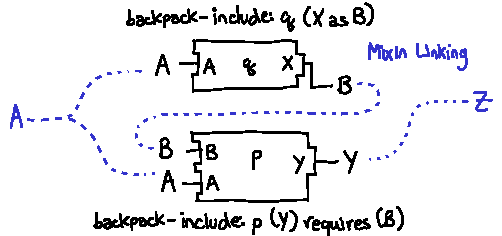
\includegraphics{diagrams/mixin-diagram.pdf}
\end{figure}

\noindent
Here, we look at the process of mixin linking \cidl{p} and \cidl{q} in
the component \cidl{r} in our running example (Figure~\ref{fig:stuff}).
The includes of \cidl{p} and \cidl{q} are represented as boxes, each of
which have an input port for every required module (\modname{A} for \cidl{q}
and \modname{A}, \modname{B} for \cidl{p}), and an output
port for every provided module (\modname{X} for \cidl{q} and \modname{Y}
for \cidl{p}).  Every port is labeled with a module name, which may
be renamed according to the \texttt{backpack-include} (e.g., \modname{X} from \cidl{q}
is renamed to \modname{B}).

These two components are linked in two ways: first, the (renamed) output
of \cidl{q} is linked to the input of \cidl{p} which has the same
\modname{B}; second, the input \modname{A} of \cidl{p}
and \cidl{q} are merged together to form a single input for \cidl{r}.
The result is a complete wiring diagram for \cidl{r}\footnote{Well, mostly
complete; \cidl{base} is omitted since it doesn't contribute in any
interesting way to linking.}:

\begin{figure}[H]
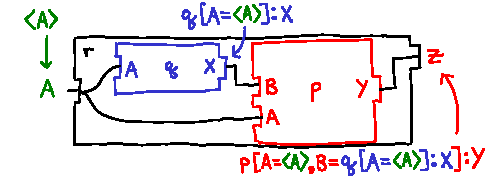
\includegraphics{diagrams/uid-diagram.pdf}
\end{figure}

\noindent
With this wiring diagram in hand, we can say what the shape of \cidl{r}
is by successively computing \emph{module identities} ($M$) and
\emph{\uid{}s} ($P$) for the modules and components defined in the
component.  In \cidl{r}, we first bind a \emph{module variable} \hv{A}
(a module identity) for our unfilled requirement \modname{A}.  \hv{A}
feeds into the input port for \cidl{q}: thus we give \cidl{q} the
\uid{} $\cidl{q}[\subst{A}{\hv{A}}]$, mapping each of its input ports (\modname{A})
to the module identity (\hv{A}) that filled it.  As \modname{X} is defined
in \cidl{q}, it then gets the module identity $\Mod{\cidl{q}[\subst{A}{\hv{A}}]}{X}$.
We continue computing identities until we know the identity of every exported
or reexported module in \cidl{r}; in this case, \modname{Y} from \cidl{p}
(which is reexported as \modname{Z}).  Then the component shape of
\cidl{r} is $\forall \hv{A}.\, \{ \prov{\modname{Z}}{\Mod{\cidl{p}[\ldots]}{Y}} \}$.

The elaborated \unit{} for \cidl{r} can be seen in Figure~\ref{fig:linked-example};
it too follows straightforwardly from the wiring diagram.  In particular,
the dependency requirements that are to be merged for signature \modname{A}
are from \cidl{p} and \cidl{q}, as is evident from the diagram.

\subsection{Ordering a \unit{}}

There is a minor step which must be done before typechecking a
\unit{}: we must \emph{order} the declarations of a \unit{} since declarations in the
earlier languages in the pipeline are unordered.  At this point,
we step into the realm of the GHC compiler, as this ordering depends
on the \texttt{import} statements within (Haskell-level) modules and
signatures.  We can define a topological ordering on declarations in a
\unit{} as follows:

\begin{itemize}
    \item Obviously, every module/signature declaration depends on
    any module/signature/dependency declaration which defines a
    module it imports.
    \item Every module declaration implicitly depends on every signature
    declaration in the component.  (This means that it is illegal for a
    signature to import a locally defined module.  In the absence of
    mutual recursion such signatures would not be implementable.)
    \item A dependency declaration $\textsf{dependency}~P$ depends
    on the signature declarations for every free module variable
    in $P$.  For example, in the definition of component \cidl{r} in
    Figure~\ref{fig:linked-example},
    \textsf{signature}~\modname{A} must precede the dependencies
    on \cidl{p} and \cidl{q}, because both mention \hv{A}; but
    can come after the \cidl{base} dependency which does not
    depend on \modname{A}.
%   \item A signature $m$ depends on another signature if it
%   transitively imports it, either locally in this module, or
%   within any of the dependencies (since dependencies there
%   merge into our local dependency).

%   A signature $m$ which is merged from $\Mod{p[S, \subst{m'}{\hv{m}}, S']}{m'}$
%   depends on the signatures of any free module variables in $S$, where $S$
%   is the set of requirements that signature $m'$ in $p$ transitively depends on.
%   This is because the required interface for this
%   component is not well-defined before we know the types of $S$.
%   \Red{Forward reference to worked example here.}
\end{itemize}
%
A dependency cycle indicates mutual recursion and is not allowed by GHC.
(In principle, other compilers might be more permissive.)

\subsection{Typechecking a \unit{}}
\label{sec:overview-compiler}


\begin{figure}
\[
\begin{array}{rcll}
  \Uunitty &::=& \forall \Theta.\, \forall \theta.\, \{\Sigma_R\} \rightarrow \{\Sigma_P\}
    & \text{Component type} \\
  \theta &::=& \overline{\hv{m.n}} & \text{Name variable quantifiers} \\
  \Sigma &::=& \overline{m : \tau}
    & \text{Provided/required types} \\
  \Gamma &::=& \overline{\Up : \Uunitty} & \text{Component typing context} \\
  &&&\\
  \tau &::=& \UobjTau{\UNs}{\overline{\Uty}} & \text{Module type} \\
  % \tau_R &::=& \exists \overline{\hv{m.n}}.\, \tau  & \text{Signature type} \\
  \UNs &::=& \overline{\UN} & \text{Export specification} \\
  \Uty &::=& \texttt{data}~n :: \I{kind} & \text{Defined entity spec} \\
       &  |& \texttt{data}~n :: \I{kind} = \cdots N \cdots& \\
       &  |& n :: \cdots N \cdots& \\
       &  |& \cdots& \\
  &&&\\
  \Un   && \multicolumn{2}{l}{\text{Haskell source-level entity name}} \\
  \UN &::=& M.\Un & \text{Original name} \\
      &|&   \nhv{m.n} & \text{Name hole} \\
  \USn &::=& \overline{\subst{m.n}{N}} & \text{Name substitution} \\
\end{array}
\]
\caption{Semantic objects of Haskell with \Backpack{}.}
%  We say $\tilde{\tau}$ to refer to the $\UNs$ of a $\tau$. Export specifications $\UNs$ have the invariant that every $n$ is distinct; so we may say $\Un \mapsto \UN \in \UNs$ to match the specific $\UN$ with $\Un$.
\label{fig:haskell-semantics}
\end{figure}

After mixin linking has produced a \unit{} definition from a \ccomp{}
definition, the component can now be \emph{typechecked} into Haskell's
semantic objects (Figure~\ref{fig:haskell-semantics}).  We now
consider how to typecheck each of the declarations in a \unit{}.
Broadly speaking, the type of a component $\Xi$ is a function type $\Sigma_R
\rightarrow \Sigma_P$, mapping from the required types
$\Sigma_R$ to the provided types $\Sigma_P$ (we'll say
more about the quantifiers shortly).

\paragraph{Typechecking a module}
A module is typechecked to produce a \emph{module
type} $\tau$, consisting of an \emph{export
specification} $\UNs$---what gets brought into scope when
you import this module---and a set of \emph{defined entity specifications}
$\overline{\Uty}$---the types and values defined by
this module.  Syntactically, these are represented with
a notation reminiscent of Haskell module declarations:
$\UobjTau{\UNs}{\overline{\Uty}}$.

For example, the module
\modname{W} in \cidl{base} (Figure~\ref{fig:linked-example}) type
checks to the following module type (also given syntactically
in Figure~\ref{fig:typing-example}):

\begin{figure}[H]
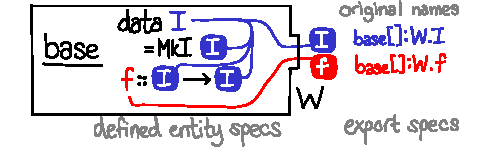
\includegraphics{diagrams/base-types.pdf}
\end{figure}

\noindent
In the diagram, the enboxed references to \texttt{I} and \texttt{f} have
been wired up to their definitions.  In other words, there are
no unresolved Haskell-source level names in a module type: all
names are resolved to \emph{original names} $N ::=
M.n$, which serve as unique identifiers for any entities; in the
diagram, this is shown by wiring them up.  An original name for an entity
defined in a module is generated by joining the identity
of the module being compiled---$\MOD{base}{}{W}$ in this case---
with the Haskell source level name (e.g., \texttt{I}, \texttt{f}).

Module types serve two key functions. First, the export
specification denotes the entities made available when resolving a
module import statement of this module.%
\footnote{ The export specification of this module type should also
  mention the data constructor \texttt{MkI}.  To simplify the
  presentation, we omit such subordinate names in export
  specifications. See the \textit{espc} semantic object of
  \OldBackpack~\cite{backpack}.  } Second, the defined entity
specification of $\MOD{base}{}{W}.\texttt{I}$ denotes the ``type'' (or
rather, the kind) of this Haskell type.  If, when typechecking
another module, we need to look up the kind of $\MOD{base}{}{W}.\texttt{I}$,
we look up the module type of $\MOD{base}{}{W}$ from the context
and then find the defined entity specification for \texttt{I}
within the module type.

\paragraph{Typechecking a signature}
Typechecking \cidl{q} (Figure~\ref{fig:linked-example}) from our running example requires
us to deal with a signature declaration.  Here is a
representation of the final type of \cidl{q}, which we can think of as
a zoomed in version of the diagram from Section~\ref{sec:overview-mixin}:

\begin{figure}[H]
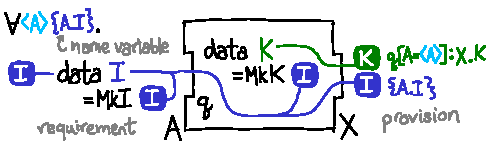
\includegraphics{diagrams/q-types.pdf}
\end{figure}

\noindent
In the diagram, the declarations from the signature are
drawn externally from \cidl{q}.  We do not know what module
will be used to fill the requirement \texttt{A}, and
consequently, we don't know what original name will provide an
implementation of \texttt{I}, although we do have a type which
it must satisfy once we do know the original names.

In mixin linking, we bound a module variable \hv{A} to represent the
unknown module identity.  In typechecking, we bind a \emph{name
variable} $\nhv{m.n}$ to represent the unknown entity $n$ required by
requirement $m$.

In theory, we typecheck a signature source file in much the same way
that we a typecheck a module, assigning a fresh name variable for each
defined entity in the signature.  In practice, we want to avoid
forcing the user to explicitly write the full requirement of the
component; rather, we'd rather infer the requirement from the local signature as well
as the dependencies of the component.  We lack a good formal model for
this process (see Section~\ref{sec:merging}), so in the formal development
in Section~\ref{sec:compiler}, we assume that the inferred requirement
type is given nondeterministically.

You may be wondering why name variables are not simply defined as
$\hv{m}.n$.  In fact, names of this form demand that $n$ be defined
by $\hv{A}$ itself, ruling out the possibility that it \emph{reexports}
$n$ from another module.

\paragraph{Typechecking a dependency}
Now we can define the key operation for typechecking in \Backpack{}:
how to compute the type of \cidl{q} instantiated with an implementation
for its requirements.  These instantiations are specified to the
compiler via \textsf{dependency} declarations.
Let's consider a simple one: filling \cidl{q}'s
requirement with \modname{W} from \cidl{base}, i.e., $\UsynDepEmpty{\cidl{q}[\subst{A}{\Mod{\cidl{base}[]}{W}}]}$.

\begin{figure}[H]
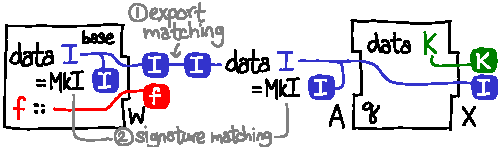
\includegraphics{diagrams/q-base-types.pdf}
\end{figure}

\noindent
There are two key steps in this diagram: first, we take the required
export specification from \cidl{q}, and the provided export specification
from \cidl{base}, and we perform \emph{export matching}, instantiating
the name variable with its true identity (diagramatically, it's
just a line.)  Obviously, you can provide more exports than you require, but
if you don't provide enough this step fails.

The second step is \emph{signature matching}: we check if the type
provided by \cidl{base} matches the required type of \cidl{q}.  This
step must occur after export matching: otherwise, we don't know that
\texttt{I}s mentioned in the constructor \texttt{MkI} are the same.

The final types of \cidl{q} are the same types as before, but now
with their module variables and name variables resolved according
to the module substitution and name matching.
What the final original names of \texttt{K}
and \texttt{I} exported by \cidl{q}?  \texttt{I} is easy: it's
just \MOD{base}{}{W}.\texttt{I}.  \texttt{K} is not too difficult either;
recall that the uninstantiated original name for \texttt{K} is
\MOD{q}{\subst{A}{\hv{A}}}{X}.\texttt{K}.  Then, applying the module
substitution $\subst{A}{\Mod{\cidl{base}[]}{W}}$ will give you the final
module name.  Alternately, just read it off the diagram!

%   \paragraph{Signature merging}
%   There is one final detail: how to merge requirements from
%   the dependencies of a component.  If
%   we know the required module types of all our dependencies, the merge is
%   straightforward.  For example, here are the module types to be merged
%   in \cidl{r} for the signature \modname{A}:
%   \[
%   \begin{array}{lll}
%   &\begin{array}{l}
%       \UobjIface\: (\MOD{base}{}{W}.\texttt{I}) \\
%   \end{array} & \text{Local signature} \\
%   \oplus&
%   \begin{array}{l}
%       \UobjIface\: (\nhv{\texttt{A.J}}) \\
%       \quad\texttt{data J :: *}
%   \end{array} & \text{From \cidl{p}} \\
%   \oplus&
%   \begin{array}{l}
%       \UobjIface\: (\nhv{\texttt{A.I}}) \\
%       \quad\texttt{data I :: * = MkI}\ \nhv{\texttt{A.I}}
%   \end{array} & \text{From \cidl{q}} \\
%   =&
%   \begin{array}{l}
%       \UobjIface\: (\MOD{base}{}{W}.\texttt{I}, \nhv{\texttt{A.J}}) \\
%       \quad\texttt{data J :: *}
%   \end{array} & \text{Final requirement for \cidl{r}}
%   \end{array}
%   \]
%   %
%   The export lists are unioned together, and we discover that \nhv{A.I}
%   actually must implemented with $\MOD{base}{}{W}.\texttt{I}$. And since
%   the entity \texttt{I} is already implemented, we additionally
%   drop its specification from the resulting requirement (having checked
%   that its specification from \MOD{base}{}{W} matches that from \cidl{q}).

%   Unfortunately, this definition of signature merging is circular: to
%   compute the instantiated type of a component, we need to know the (full)
%   types of our requirements; but to compute the type of a merged
%   requirement, we need to compute the instantiated types of the components
%   which merge into the requirement. \Scott{I'm not sure what this means. Can
%   you identify how the problem manifests in the example so far?}
%   The solution to this problem is to
%   define \emph{partial instantiation}, which only instantiates a component
%   type as much as is necessary to determine the type of the requirement in
%   question.  We give the technical details in Section~\ref{sec:compiler}.

%   \paragraph{Compiling instantiated components}
%   \Red{Need to rewrite this section, motivate why the semantics split
%   into separate type checking and compiler.}
%   When a \unit{} has no
%   requirements, it can be compiled.  In this case, compilation is very
%   trivial: the dependencies of \unit{}s can be successively instantiated
%   by Cabal to form a graph of instantiated components, which GHC can
%   simply compile in order.  In this way, the soundness of Haskell with \Backpack{}
%   trivially reduces to the soundness of Haskell without \Backpack{}.

%   While compilation of \Backpack{} is trivially sound, we would like to
%   relate type checking and compilation with a property that says that if a
%   unit typechecks compositionally, it also typechecks monolithically
%   (i.e., when you re-typecheck the entire transitive closure.)
%   Unfortunately, in full Haskell it is impossible for this to be the case
%   with our current signature language and semantics.  In Section \Red{XXX}
%   we give some examples and conjecture under what circumstances this
%   property does hold.


\subsection{Instantiation and compilation}
\label{sec:overview-instantiate}

Typechecking is all very well and good, but what about
running our programs?  For both soundness reasons (Section~\ref{sec:limitations})
and performance reasons, it is desirable to defer compiling
until we know how all the requirements of a component are to be
filled.

When we have a \unit{} which has no unfilled requirements,
the package manager computes the
\emph{instantiated component graph}, reflecting all of the
concrete code dependencies of the component.  Specifically, given a closed instantiated component identity $p[S]$, for every
\textsf{dependency} $P$ of $p$'s mixed component, recursively
instantiate $\substw{P}{S}$.  Furthermore, for every $\substMod{m}{P}{m'} \in S$,
recursively instantiate $P$.  Then, we compile each instantiated component
in topological order.  This compilation is exactly like ordinary
compilation without \Backpack. The only new feature is that signatures
compile into trivial module which reexport entities from
the backing implementation; otherwise, modules that imported the signature might see
entities from the backing implementation that were not exported by the
signature.

It is important that the package manager computes
the instantiated component graph: \emph{applicative}
semantics of instantiation mean that completely independent
components could instantiate a library in the same way: in such
cases we should share the compiled code.  A traditional compiler cannot
do this: it is solely responsible for transforming source
files into object code.











%%% Local Variables:
%%% mode: latex
%%% TeX-master: "paper"
%%% End:
